% !TEX root = ../Dokumentation.tex
\subsection{Energieversorgung}

\textbf{Funktionsbeschrieb}\\[0.2cm]
Das autonome Entsorgungsfahrzeug muss mit Energie versorgt werden. Dazu werden Akkumulatoren eingesetzt, welche das Gerät während dem gesamten Einsatz mit Strom versorgen. 
\\[0.2cm]
\textbf{Komponentenbeschrieb}\\[0.2cm]
\begin{figure}[h]
	\centering
	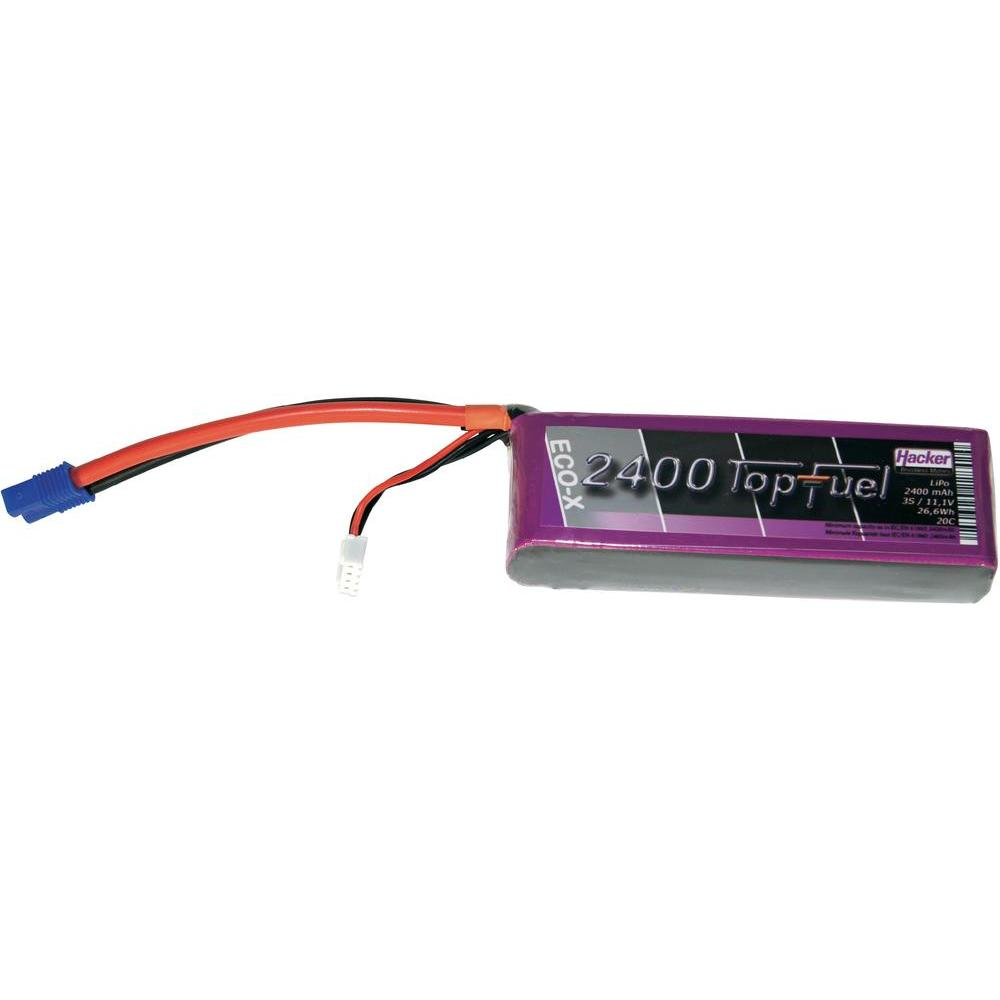
\includegraphics[width=0.5\textwidth]{./Images/Lipo.JPG}
	\caption{2400 mA/h Lipo  (Quelle:http://www.conrad.ch/ce/)}
	
\end{figure}
Um Störungen, die z.B durch den erhöten Anlaufstrom der Motoren verursacht werden könnten, zu vermeiden, werden die intelligenten Systeme (Microcontroller, Mini-Computer,etc.)möglichst getrennt von den Motoren gespiesen. Dazu wird einerseits ein 11.1Volt Lithium-Polymer-Akkumulator für die Motoren verwendet und andererseits ein 7.4 Volt Lipo für die empfindlichen Systeme. Beide werden voraussichtliche eine Kapazität zwischen 1800 und 3000 mA/h vorweisen.
 \\[0.2cm]
\textbf{Begründung}\\
Lithium-Polymer-Akkumulatoren haben im Vergleich zu anderen die höchste Energiedichte und den kleinsten 
\textbf{Berechnungen}
\textbf{Testergebnisse}